\documentclass[hyperref={unicode}]{beamer}
\usepackage[utf8]{inputenc}
\usepackage[IL2]{fontenc}
\usepackage[czech]{babel}
\usepackage{amsmath}
\usepackage{amsthm}
\usepackage{amsfonts}
\usepackage{graphicx}
\usepackage[hypcap=false]{caption}
\usepackage{etoolbox}
\usepackage{lmodern}

\usetheme[pageofpages=z,% String used between the current page and the total page count.
          bullet=circle,% Use circles instead of squares for bullets.
          titleline=true,% Show a line below the frame title.
          alternativetitlepage=true,% Use the fancy title page.
          %titlepagelogo=logo-fit,% Logo for the first page.
          %% Watermark used in every page.
          %watermarkheight=50px,% Height of the watermark.
          %watermarkheightmult=4,% The watermark image is 4 times bigger
          ]{Torino}



\makeatletter
\pretocmd{\section}{\addtocontents{toc}{\protect\addvspace{5\p@}}}{}{}
\pretocmd{\subsection}{\addtocontents{toc}{\protect\addvspace{5\p@}}}{}{}
\makeatother

\setbeamertemplate{section in toc}[circle]
\setbeamertemplate{subsection in toc}[ball]
\setbeamertemplate{subsection in toc}
{\leavevmode\leftskip=2em$\bullet$\hskip1em\inserttocsubsection\par}

\setbeamercolor{section in toc}{fg=black}
\setbeamercolor{subsection in toc}{fg=black}



\author{\Large{Martin Chládek}}
\title{\Huge{Konečné automaty}}
\institute{\small{Vysoké učení technické\\Fakulta informačních technologií}}
\date{\today}

\begin{document}

\watermarkoff

\begin{frame}[t,plain]
\maketitle
\end{frame}

\begin{frame}{Osnova}
\begin{minipage}{\textwidth}
       \tableofcontents
    \end{minipage}
\end{frame}

\section{Definice}
\begin{frame}[t]{Definice konečného automatu (KA)}
\begin{itemize}
    \item Model systému, který může nabývat konečně mnoho vnitřních stavů.
    \item Tento stav se mění na základě jednoduchého vnějšího podnětu.
    \item Pro daný stav je jednoznačně určeno do jakého stavu systém přejde.
    \item Vnější pozorovatel nevidí vnitřní stavy automatu, může pozorovat pouze jednoduchou dvoustavovou informaci:
    \begin{itemize}
        \setlength\itemsep{0.7em}
        \item přijímací stav automatu
        \item nepřijímací stav automatu
    \end{itemize}
\end{itemize}
\end{frame}

\section{Rozdělení}
\begin{frame}[t]{Rozdělení}
\begin{itemize}
    \setlength\itemsep{1em}
    \item Deterministický konečný automat
    \begin{itemize}
        \item Vždy se nachází právě v jednom ze svých vnitřních stavů.
    \end{itemize}
    \item Nedeterministický konečný automat
    \begin{itemize}
        \item Může se v jednu chvíli náchazet v celé množině svých vnitřních stavů.
    \end{itemize}
\end{itemize}
\end{frame}

\section{Deterministický automat}
\begin{frame}[t]{Definice deterministického konečného automatu}
\begin{itemize}
    \item Konečný automat je dán pěticí parametrů $(Q,\Sigma,\delta,q_{0},F)$, kde \hspace{3cm}
    \begin{itemize}
        \setlength\itemsep{0.7em}
        \item $Q$ je konečná neprázdná množina stavů
        \item \alt<2->{\color{black}$\Sigma$ je abeceda (konečná nožina symbolů/písmen)}{\color{gray}$\Sigma$ je abeceda (konečná nožina symbolů/písmen)}
        \item \alt<3->{\color{black}$\delta : Q\times\Sigma\to Q$ je přechodová funkce}{\color{gray}$\delta : Q\times\Sigma\to Q$ je přechodová funkce}
        \item \alt<4->{\color{black}$q_{0} \in Q$ je počáteční stav}{\color{gray}$q_{0} \in Q$ je počáteční stav}
        \item \alt<5->{\color{black}$F \subseteq Q$ je neprázdná množina přijímajících stavů}{\color{gray}$F \subseteq Q$ je neprázdná množina přijímajících stavů}
    \end{itemize}
\end{itemize}
\end{frame}

\section{Nedeterministický automat}
\begin{frame}[t]{Definice nedeterministického konečného automatu}
\begin{itemize}
    \item Nedeterministický KA je uspořádaná pětice  $(Q,\Sigma,\delta,I,F)$, kde \hspace{3cm}
    \begin{itemize}
        \setlength\itemsep{0.7em}
        \item $Q$ je konečná neprázdná množina stavů
        \item \alt<2->{\color{black}$\Sigma$ je abeceda (konečná nožina symbolů/písmen)}{\color{gray}$\Sigma$ je abeceda (konečná nožina symbolů/písmen)}
        \item \alt<3->{\color{black}$\delta : Q\times(\Sigma\cup\{\varepsilon\}\to 2^{Q}$ je (nedeterministická) přechodová funkce}{\color{gray}$\delta : Q\times(\Sigma\cup\{\varepsilon\}\to 2^{Q}$ je (nedeterministická) přechodová funkce}
        \item \alt<4->{\color{black}$I \subseteq Q$ je neprázdná množina počátečních stavů}{\color{gray}$I \subseteq Q$ je neprázdná množina počátečních stavů}
        \item \alt<5->{\color{black}$F \subseteq Q$ je neprázdná množina přijímajících (koncových) stavů}{\color{gray}$F \subseteq Q$ je neprázdná množina přijímajících (koncových) stavů}
    \end{itemize}
\end{itemize}
\end{frame}

\section{Reprezentace}
\subsection{Tabulka přechodové funkce}
\begin{frame}[t]{Možnosti reprezentace (1/6)}
\begin{itemize}
    \item Tabulka přechodové funkce \vspace{1em}
    \begin{itemize}
        \setlength\itemsep{0.7em}
        \item Stavy jsou uvedeny v záhlaví řádků.
        \item Znaky ze vstupní abecedy jsou uvedeny v záhlaví sloupců.
        \item Přechodová pravidla jsou dána obsahem vnitřních polí tabulky.
    \end{itemize}
\end{itemize}
\end{frame}

\begin{frame}{Možnosti reprezentace (2/6)}
\begin{table}[h]
\begin{center}
    \scalebox{1.5}{
    \begin{tabular}{|c|c|c|}
    \hline
         \textbf{Stav} & 0 & 1 \\ \hline
         \textbf{$S_{0}$} & $S_{0}$ & $S_{1}$ \\ \hline
         \textbf{$S_{1}$} & $S_{2}$ & $S_{0}$ \\ \hline
         \textbf{$S_{2}$} & $S_{1}$ & $S_{2}$ \\ \hline
    \end{tabular}}
    \vspace{1em}
    \caption{Příklad tabulky přechových funkcí}
\end{center}
\end{table}
\end{frame}

\subsection{Graf automatu}
\begin{frame}[t]{Možnosti reprezentace (3/6)}
\begin{itemize}
    \item Graf automatu (stavový diagram) \vspace{1em}
    \begin{itemize}
        \setlength\itemsep{0.7em}
        \item Uzly znázorňují stavy.
        \item Ohodnocené orientované hrany představují přechodové funkce.
        \item Znaky, kterými jsou hrany ohodnoceny, tvoří vstupní abecedu.
    \end{itemize}
\end{itemize}
\end{frame}

\begin{frame}{Možnosti reprezentace (4/6)}
\begin{center}
    \scalebox{0.55}{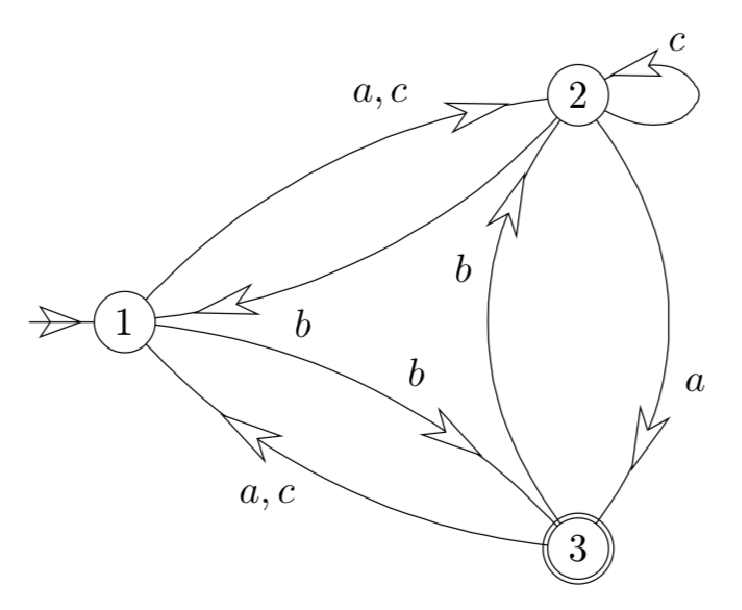
\includegraphics{stavovy-diagram.eps}}
    \captionof{figure}{Příklad grafu konečného automatu}
\end{center}
\end{frame}

\subsection{Stavový strom}
\begin{frame}[t]{Možnosti reprezentace (5/6)}
\begin{itemize}
    \item Stavový strom\vspace{1em}
    \begin{itemize}
        \setlength\itemsep{0.7em}
        \item Moc se nepoužívá.
        \item Kořen stromu představuje počáteční stav.
        \item Z každého uzlu (nesmí být listem stromu) vychází tolik hran, kolik má odpovídající stav následníků.
        \item Pokud je stav reprezentován více uzly, pak hrany vycházejí pouze z prvního uzlu.
    \end{itemize}
\end{itemize}
\end{frame}

\begin{frame}{Možnosti reprezentace (6/6)}
\begin{center}
    \scalebox{0.45}{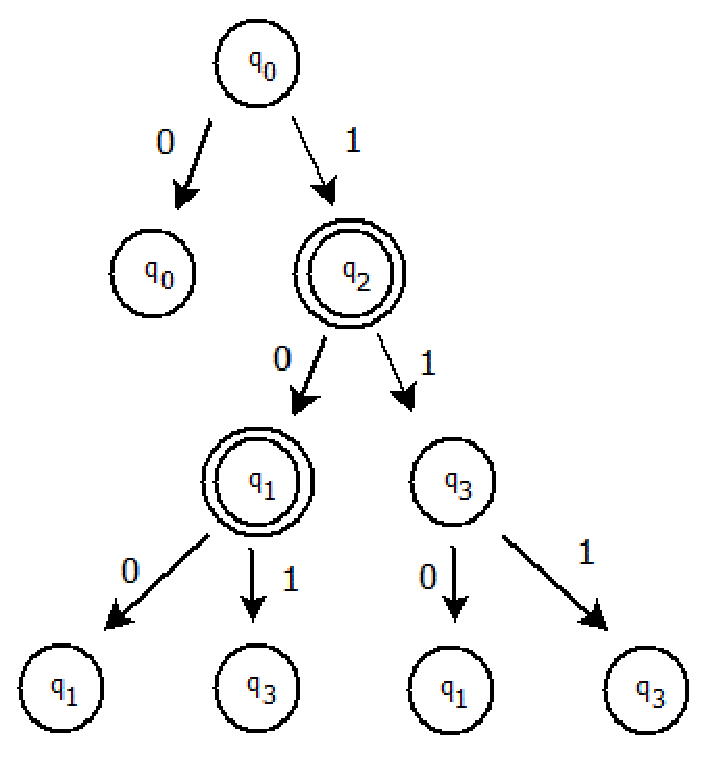
\includegraphics{stavovy-strom.eps}}
    \captionof{figure}{Příklad stavového stromu konečného automatu}
\end{center}
\end{frame}

\begin{frame}[t]{Použité zdroje}
\begin{itemize}
        \setlength\itemsep{1em}
        \item Deterministický konečný automat\\
        {\footnotesize \url{http://www.cs.vsb.cz/kot/soubory_animaci/a-definice_dfa.pdf}}
        \item Konečný automat\\
        {\footnotesize \url{http://voho.eu/wiki/konecny-automat/}}
        \item Vizualizace práce konečných automatů\\
        {\footnotesize \url{https://www.vutbr.cz/www_base/zav_prace_soubor_verejne.php?file_id=116647}}
        \item Úvod do teoretické informatiky\\
        {\footnotesize \url{https://www.fi.muni.cz/~hlineny/Vyuka/Old/UTI-distext05.pdf}}
\end{itemize}
\end{frame}

\begin{frame}[t]{Použité zdroje}
    \begin{itemize}
        \setlength\itemsep{1em}
        \item Konečný automat\\
        {\footnotesize \url{https://matematika.cz/konecny-automat}}
        \item Reprezentace konečných automatů\\
        {\footnotesize \url{http://lucie.zolta.cz/index.php/zaklady-teoreticke-informatiky/13-konecne-automaty/5-reprezentace-konecnych-automatu}}
    \end{itemize}
\end{frame}

\end{document}

